%%%%%%%%%%%%%%% Start of Title Page %%%%%%%%%%%
\begin{titlepage}
\begin{center}
\textit{Heaven's Light is Our Guide}
\\[0.5cm]
\textbf{\Large Rajshahi University of Engineering \& Technology}
\\[0.3cm] 
\textbf{\large Department of Electronics \& Telecommunication Engineering}
\\[0.2cm]
\begin{figure}[!htbp]
    \centering
    
\includegraphics[scale=0.3]{Figures/logo_ruet}
    \label{fig:RUET logo}
\end{figure}
\textbf{\Large EEE1254: Sessional Based on EEE1253 }
\\[0.5cm]
\myrule[1pt][5pt]

%%%%%%%%%%%%%%%%%%%%%%%%%%%%%%%%%%%%%%%%%%%%%%%
%%%%%%%%%%%%%%% STUDENT'S INFO %%%%%%%%%%%%%%%%
%%%%%%%%%%%%%%%%%%%%%%%%%%%%%%%%%%%%%%%%%%%%%%%

\textbf{\Large  Experiment No. \ref{exp3}}
\\[.25cm]
\textbf{\large Study of External Characteristics Curve of a DC Shunt, Cumulative and Differential Compound Generator.}
\\ 
\myrule[1pt][5pt] 
\begin{minipage}{0.4\textwidth}
\vspace{0.5cm}
\begin{flushleft} 
\emph{\textbf{\large Submitted by:}}
\\
Antu Roy Chowdhury \\
Roll: 2004011 \\
Session: 2020-21
\end{flushleft}
\end{minipage}
~
\begin{minipage}{0.4\textwidth}
\vspace{0.5cm}
\begin{flushright} 
\emph{\textbf{\large Submitted to:}} 
\\
A. S. M. Badrudduza
\\
Assistant Professor
\\
Dept. of ETE, RUET
\\
\end{flushright}
\end{minipage}\\[0.7cm]
\makeatother

\textbf{Date of Experiment : 11/10/2022}\\
\textbf{Date of Submission : 18/10/2022}\\[1cm]

%************** End of Student's Info *********


\vfill
%%%%%%%%%%%%%%% TEACHER SECTION %%%%%%%%%%%%%%%
\hrulefill
\vspace{-5mm}
\begin{multicols}{3}
\begin{itemize} [labelindent=3em,labelsep=0.5cm,leftmargin=*,noitemsep]
        \item[] \textbf{\underline{Report}}
        \item[$\square$] Excellent
        \item[$\square$] Very Good
        \item[$\square$] Good
        \item[$\square$] Average
        \item[$\square$] Poor
\end{itemize}
\columnbreak
\textbf{(Teacher's Section)}
\\[1.5cm]
--------------------------------
\\
Signature
\columnbreak
\begin{itemize}
[labelindent=6em,labelsep=0.5cm,leftmargin=*,noitemsep]
        \item[] \textbf{\underline{Viva}}
        \item[$\square$] Excellent
        \item[$\square$] Very Good
        \item[$\square$] Good
        \item[$\square$] Average
        \item[$\square$] Poor
\end{itemize}
\end{multicols}
\end{center}
\end{titlepage}
\newpage
%************** End of Teacher Section ********
%************** End of Title Page *************


%%%%%%%%%%%%%%% Exp. Positioning %%%%%%%%%%%%%%
\titleformat{\chapter}[display]
  {\normalfont\large\bfseries}{\chaptertitlename\ \thechapter}{0pt}{\large}
\titlespacing*{\chapter}{0pt}{-15pt}{10pt}
% \addcontentsline{lof}{chapter}{\protect\numberline{ \ref{exp1}}}
% \addcontentsline{lot}{chapter}{\protect\numberline{ \ref{exp1}}}
%************** End of Exp. Positioning *******


%%%%%%%%%%%%%%%%%%%%%%%%%%%%%%%%%%%%%%%%%%%%%%%
%%%%%%%%%%%%%%% Student's Part %%%%%%%%%%%%%%%%
%%%%%%%%%%%%%%% Start of Report %%%%%%%%%%%%%%%
%%%%%%%%%%%%%%%%%%%%%%%%%%%%%%%%%%%%%%%%%%%%%%%


%**********************************************
\chapter{Study of External Characteristics Curve of a DC Shunt, Cumulative and Differential Compound Generator.}
\label{exp3}


%**********************************************
\section{Objectives}
The main objectives of this experiment are
\begin{itemize}
    \item To understand the characteristics of DC shunt, Cumulative and Differential Compound Generator.
    \item To learn the characteristics curve of DC shunt, Cumulative and Differential Compound Generator.
    \item To know the differences between DC shunt, Cumulative and Differential Compound Generator.
    \item To know about the usage of DC shunt, Cumulative and Differential Compound Generator in different fields.
\end{itemize}


%**********************************************
\section{Theory}
In a shunt generator, the field winding is connected in parallel with the armature winding so that the terminal voltage of the generator is applied across it. For a shunt generator the initial voltage is zero. For the residual Magnetism a small amount of flux is generated then it is followed by generating a small amount of current. Because of presence of small residual flux in the field poles, DC Shunt Generator will have a small voltage at its terminal even though the switch is open when driven at rated speed. This is called the voltage build up process of a shunt generator. The major disadvantage of a DC shunt Generator is if the load current is increased then the terminal voltage drop also increases. Because of the voltage loss in the line as well as the generator's terminal voltage decreasing with increasing load, its use is not suitable for sending power to distantly positioned places. The formula for the terminal voltage for either the short shunt or long shunt is 
\begin{equation}
    \nonumber
    V_t = E_g - I_aR_a - I_sR_g
\end{equation}
Here,
\begin{align}
    \nonumber
    V_t\hspace{0.1cm} =\hspace{0.1cm} Terminal\hspace{0.1cm} Voltage
    \\\nonumber
    I_a\hspace{0.1cm} =\hspace{0.1cm} Armature\hspace{0.1cm} Current
    \\\nonumber
    R_a \hspace{0.1cm}= \hspace{0.1cm}Armature\hspace{0.1cm} circuit\hspace{0.1cm} resistance
    \\\nonumber
    I_s\hspace{0.1cm} =\hspace{0.1cm} Series\hspace{0.1cm} field\hspace{0.1cm} resistance
    \\\nonumber
    E_g \hspace{0.1cm}=\hspace{0.1cm} Generated\hspace{0.1cm} voltage
\end{align}
\FloatBarrier
Around the core of each pole there are two sets of windings. One winding contains many turns of fine wire, which, of course, is the shunt-field winding. The second winding, the series-field winding, consists of few turns of heavy wire. The heavy wire is necessary because the load current flows through the series field. The effect of this additional to the flux of the shunt field. The effect of this additional flux gives the compound generator its own particular characteristics.  It is possible to reverse the direction of current in the series field so that the flux of the series field opposes the flux of the shunt field. This is accomplished by interchanging the series-field connections. With this connection the generated voltage at no load would be the same as for the shunt generator because the series field produces no flux. When load is applied, load current flows through the series filed, setting up lines of flux that oppose the flux of the shunt field. The net flux cut by the armature conductors is less than the flux at no load resulting in a lower induced voltage. Since induced voltage is less, the terminal voltage will also be less. The differential compound generator is the name applied to the compound generator where the series-field flux opposes the shunt-field flux.
\begin{figure}[hbt!]
\vspace{00mm}
    \centerline{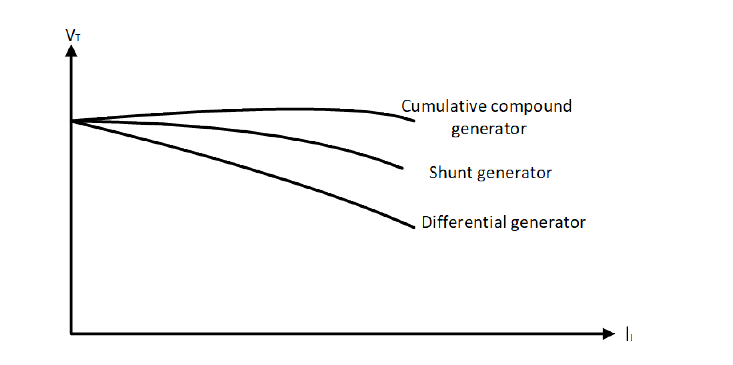
\includegraphics[width=1\textwidth]{Figures/Exp03/image_2022-10-17_220525721.png}}
    \vspace{0mm}
    \caption{Comparison of external characteristics curve of a DC Shunt, Cumulative and Differential Compound Generator.}
    \label{fig:figg1}
\end{figure}
\newpage


%**********************************************
\section{Required Apparatus}
\begin{enumerate}
\item DC Supply
\item Multimeter
\item Resistor (107 Ohm)- 2 pieces
\item Voltmeter (0-450 V). 
\item Ammeter (0-2 A , 0-10A) - 2-pieces.
\item Connecting wire
\item Generator (240V, 18A, $I_f$= 9.1/4.55
\end{enumerate}

\newpage

%**********************************************
\section{Circuit Diagram}

\begin{figure}[hbt!]
\vspace{00mm}
    \centerline{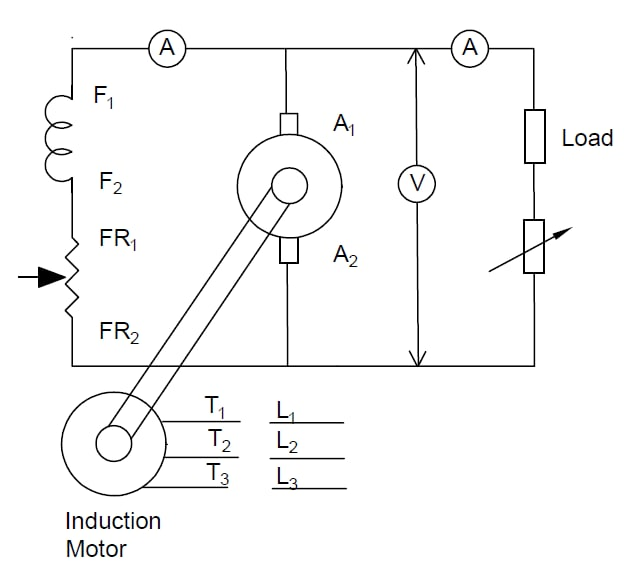
\includegraphics[width=0.6\textwidth]{Figures/Exp03/dcshunt.jpeg}}
    \vspace{0mm}
    \caption{Circuit diagram for DC Shunt Generator with Load}
    \label{fig:figg2}
\end{figure}
\begin{figure}[hbt!]
\vspace{00mm}
    \centerline{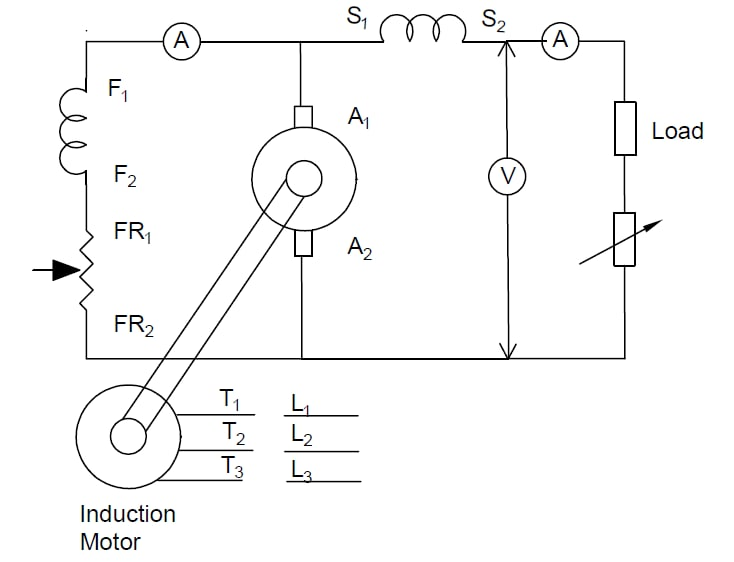
\includegraphics[width=0.6\textwidth]{Figures/Exp03/cumulative.jpeg}}
    \vspace{0mm}
    \caption{Circuit diagram for cumulative compound generator}
    \label{fig:figg2}
\end{figure}
\begin{figure}[hbt!]
\vspace{00mm}
    \centerline{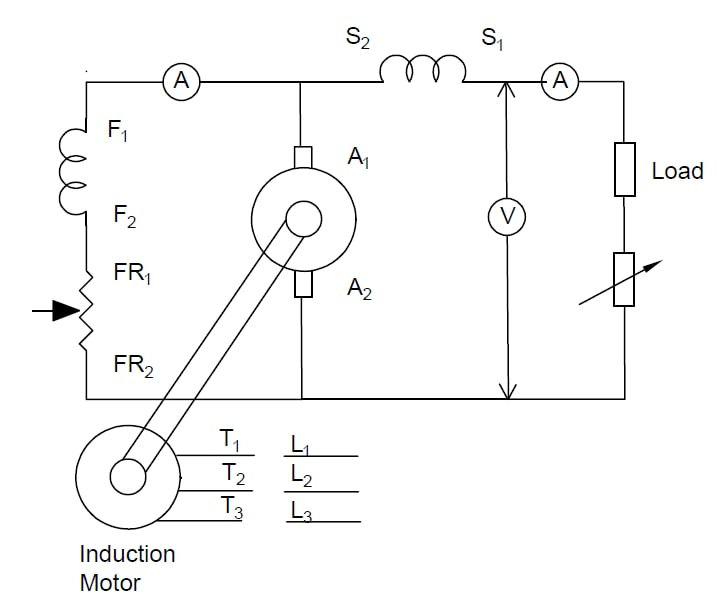
\includegraphics[width=0.6\textwidth]{Figures/Exp03/differtial.jpeg}}
    \vspace{0mm}
    \caption{Circuit diagram for differential compound generator}
    \label{fig:figg2}
\end{figure}
%**********************************************
\FloatBarrier
\section{Procedure}
\begin{itemize}
    \item All the connections of the wires were given as in fig 3.2.
    \item The switch of the induction motor was turned on, the rotation was checked. If the rotation was not found accurately then any two connections between $T_1, T_2, T_3,$ was interchanged to fix the rotation. 
    \item The rheostat was fixed at a high amount of resistance and then the value of resistance was gradually decreased.
    \item After increasing the voltage to the generator's rated voltage by adjusting the field rheostat, readings from the Ammeter and Voltmeter under no load conditions were recorded to the data table.
    \item The load was gradually changed and voltmeter and ammeter values were recorded for each load.
    \item The generator was unloaded, the field rheostats of the DC shunt generator and motor were removed to their maximum and minimum positions respectively and the supply voltage switch was opened.
    \item The steps from 1 to 5 were repeated after making a new connection as shown in fig 3.3 and 3.4
    \item The readings were turned plotted into a table and a graph was drawn.
\end{itemize}

%**********************************************




%**********************************************

\section{Data Table}
\begin{table}[hbt!]
\centering
\caption{No load magnetization of a separately excited DC generator}
\label{tab1}
% Please add the following required packages to your document preamble:
% \usepackage{multirow}

\begin{tabular}{|c|c|cc|cc|cc|}
\hline
\multirow{2}{*}{\begin{tabular}[c]{@{}c@{}}No. of\\ Obs.\end{tabular}} & \multirow{2}{*}{\begin{tabular}[c]{@{}c@{}}Load \\ Current, $I_L$ (A)\end{tabular}} & \multicolumn{2}{c|}{DC Shunt Generator} & \multicolumn{2}{c|}{\begin{tabular}[c]{@{}c@{}}Cumulative Compund\\ Generator\end{tabular}} & \multicolumn{2}{c|}{\begin{tabular}[c]{@{}c@{}}Differential Compund\\ Generator\end{tabular}} \\ \cline{3-8} 
                                                                      &                                                                                  & \multicolumn{1}{c|}{$V_T$ (V)}   & $I_f$ (A)  & \multicolumn{1}{c|}{$V_T$ (V)}                             & $I_f$ (A)                            & \multicolumn{1}{c|}{$V_T$ (V)}                              & $I_f$ (A)                             \\ \hline
1                                                                     & 0                                                                                & \multicolumn{1}{c|}{230}      & 0.46    & \multicolumn{1}{c|}{230}                                & 0.46                              & \multicolumn{1}{c|}{230}                                 & 0.46                               \\ \hline
2                                                                     & 1                                                                                & \multicolumn{1}{c|}{218}      & 0.44    & \multicolumn{1}{c|}{234}                                & 0.447                             & \multicolumn{1}{c|}{208}                                 & 0.43                               \\ \hline
3                                                                     & 1.175                                                                            & \multicolumn{1}{c|}{216}      & 0.43    & \multicolumn{1}{c|}{224}                                & 0.44                              & \multicolumn{1}{c|}{204}                                 & 0.415                              \\ \hline
4                                                                     & 1.375                                                                            & \multicolumn{1}{c|}{214}      & 0.425   & \multicolumn{1}{c|}{222}                                & 0.435                             & \multicolumn{1}{c|}{198}                                 & 0.41                               \\ \hline
5                                                                     & 1.575                                                                            & \multicolumn{1}{c|}{210}      & 0.42    & \multicolumn{1}{c|}{223}                                & 0.43                              & \multicolumn{1}{c|}{194}                                 & 0.40                               \\ \hline
6                                                                     & 1.775                                                                            & \multicolumn{1}{c|}{208}      & 0.41    & \multicolumn{1}{c|}{220}                                & 0.43                              & \multicolumn{1}{c|}{188}                                 & 0.38                               \\ \hline
7                                                                     & 1.975                                                                            & \multicolumn{1}{c|}{206}      & 0.405   & \multicolumn{1}{c|}{218}                                & 0.42                              & \multicolumn{1}{c|}{186}                                 & 0.37                               \\ \hline
8                                                                     & 2.2                                                                              & \multicolumn{1}{c|}{204}      & 0.4     & \multicolumn{1}{c|}{216}                                & 0.405                             & \multicolumn{1}{c|}{170}                                 & 0.35                               \\ \hline
\end{tabular}

\end{table}



%**********************************************
\FloatBarrier
\newpage
\section{Result} 
\begin{figure}[hbt!]
\vspace{0mm}
    \centerline{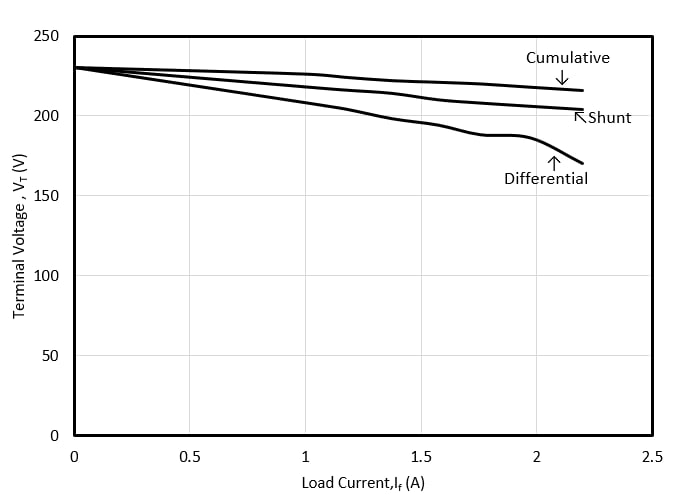
\includegraphics[width=1.2\textwidth]{Figures/Exp03/result.jpeg}}
    \vspace{0mm}
    \caption{Comparison of external characteristics curve of a DC Shunt, Cumulative and Differential Compound Generator.}
    \label{fig:figg3}
\end{figure}
\vspace{20mm}




%**********************************************
\FloatBarrier
\section{Discussions and Conclusion}

In this experiment the differences and the external characteristics curve of a DC Shunt, Cumulative and Differential Compound Generator was observed and learned. While doing the experiment the load resistance was taken at a maximum value. The starting voltage for all the generators were kept same and it was started from 230 volts. The highest $I_f$ for DC shunt generator which was found at 230 volts was 0.46 ampere and for cumulative compound and differential generator the current was same. But lowest value of the current for these three generators were 0.4,0.405, 0.35 ampere respectively. While making the circuits a proper distance was maintained as a high voltage passed through the circuits. To make the circuit of the differential compound from cumulative compound generator only the position of $S_1$ and $S_2$ was exchanged

It was seen from the experiment that the curve for the differential compound generator was lower than the DC shunt and the cumulative compound generator was higher than DC Shunt and Differential Generator. it was expected from the theory. The decreasing rate of voltage was not same for these three types of generator which made this difference in the curve possible. So it can be said that the main objectives of the experiment were successfully completed. 



%%%%%%%%%%%%%%% Bibliography %%%%%%%%%%%%%%%%%%
%%%%%%%%%%%%%%% Uncomment only if you need %%%%
% If you need any citations then follow this:
% An article \cite{anarticle}\\
% A book \cite{abook}\\
% A series \cite{bookseries}\\
% Someone's thesis \cite{thesis}\\
% Some technical report \cite{report}\\
% A collection \cite{collection}\\
% Visited website \cite{website}\\
% Accepted for publication \cite{acceptedpub}\\
% Submitted for publication \cite{unpub}\\
% Not published \cite{notpub}\\
% Conversation \cite{conv}
% \addcontentsline{toc}{chapter}{\bibname}
% \bibliographystyle{IEEEtran} 
% \bibliography{asmbbiblio}
%************** End of Bibliography ***********



%**********************************************
%************** End of Student's Part *********
%************** End of the Report *************
%**********************************************